\section{Experiments}
\label{sec:experiments}

To evaluate the effectiveness of these ensemble strategies in maximizing explanation similarity between ensembles, we conduct a series of experiments spanning five benchmark financial datasets, three similarity metrics (each with a focus on distinct aspects of explanation similarity), and three common explanation methods. In this section, we outline the technical details involved. In~\S\ref{subsec:experiments_weight}, we perform ablations to understand the impact of local weight perturbations on explanation similarity. In~\S\ref{subsec:experiments_ensemble} we, showcase the merits of both methods in maximizing the expected explanation similarity between any two ensembles constructed from $n$ samples of the underspecification set, improvements attained without compromising test accuracy. Our experiments were conducted in Python~\citep{van1995} on standard consumer-grade CPUs,\footnote{Specifically, an 8-core Apple M1 Pro chip and a 12-core/24-thread AMD Ryzen 9 5900X processor.} parallelized with \verb+joblib+~\citep{joblib2020}. 

\paragraph{Datasets} We use five publicly available financial datasets: the Home Equity Line of Credit (HELOC)~\citep{heloc} and German Credit~\cite{uci2017} datasets both measure forms of credit risk, given input information regarding a loanee; Adult Income~\citep{uci2017} is used to predict whether a person's salary exceeds a threshold of \$50,000; Default Credit~\citep{yeh2009} and Give Me Some Credit (GMSC)~\citep{gmsc} involve predicting the likelihood of a borrower defaulting on a loan, based on a variety of financial and personal features. For each dataset, we encode negative outcomes (high risk, low salary, defaults, etc.) as $y=0$, and compute explanations with respect to the positive class, to model typical scenarios whereby users seek advice from model explanations on how to obtain a desired outcome $y=1$. Categorical features are one-hot encoded, and data is normalized to zero mean and unit variance, in part to ensure that top-$k$ feature explanations are meaningful, and not skewed towards features with smaller ranges. We fix a split of 80\% of each dataset for training, and 20\% to evaluate explanations and test accuracy. Full implementation details are provided in Appendix~\ref{subapp:datasets}.

\paragraph{Model selection} In our experiments, we use \verb+PyTorch+~\citep{paszke2019} to implement feedforward neural networks in  with fixed architectures: hidden layers of size 128, 64, and 16 are used, to provide sufficient capacity for the networks to capture largely diverse, but equally performing functional solutions. We use ReLU activations for the intermediate layers and Softmax for the output. Model selection sweeps are performed with \verb+RayTune+ \citep{liaw2018}, to identify the best performing model hyperparameters for a given dataset. Optimal hyperparameters and full implementation details are included in Appendix~\ref{subapp:models}.

To explore the underspecification set, we proceed to train 1000 models using the optimal set of hyperparameters found, changing only the random seed that controls the initialization of each neural network in weight space. We decide against randomly shuffling the training data between epochs, focusing on the effect of underspecification solely in terms of the random initialization. Notably, we also do not employ practices such as weight decay or dropout, as these techniques could limit the expressivity of the models and consequently constrain the variability of explanations, thereby obscuring our ability to test the effectiveness of ensembling strategies in aligning diverse explanations.


\paragraph{Explanations} We experiment with three common explanation methods. Input gradients, or Saliency~\citep{simonyan2013}, Smoothgrad~\citep{smoothgrad2017}, and DeepSHAP~\citep{lundberg2017}. Specifically, we seek to verify if our method offers benefits beyond those provided by Smoothgrad, given its conceptual similarity to weight perturbation. Given the widespread use of SHAP, particularly in financial domains, we experiment on DeepSHAP, %an enhanced version of DeepLIFT \citep{shrikumar2019}
which uses a selection of background samples to approximate the conditional expectations of SHAP, described in \citet{lundberg2017}. In the interests of compute, we limit the number of test inputs being explained with DeepSHAP to 100. We note that the same train/test samples are used for a given dataset, and that DeepSHAP values reached convergence, eliminating any potential source of variation in explanations that might distort the evaluation of our ensemble methods.

\paragraph{Explanation similarity metrics} We are interested in comparing the explanations provided by two models for a given input, and adopt existing top-$k$ metrics to cover distinct forms of agreement. Each metric takes a pair of top-$k$ feature sets corresponding to the two explanations.

\textit{Sign-Agreement (SA)} computes the fraction of top-$k$ features that appear in both explanations and share the same sign \citep{krishna2022}, and can be viewed as the overlap between two top-$k$ explanations, after accounting for the direction of features (whether they contributed positively or negatively to the model's prediction). We modify two other metrics taken from \cite{brunet2022}: 

\textit{Signed-Set Agreement (SSA)} is binary (per-sample), and is 1 when the two model's top-$k$ feature sets contain the same features and the features have the same signed value (the order of the top-$k$ features does not matter). SSA is thus a stricter form of SA, and is satisfied if and only if SA evaluates to 1.

\textit{Consistent Direction of Contribution (CDC)} is also binary (per-sample) and requires that any feature that appears in the top-$k$ of one model has the same signed value if it appears in the other model. CDC estimates the likelihood of a top-$k$ explanatory feature changing its contribution direction when switching between pairs of roughly equivalent models. Such changes can be confusing for end users.

\paragraph{Mode connectivity implementation} We implement mode connectivity following the method outlined in \citet{garipov2018}. This process involves training a curve between two endpoints, which, while beneficial, introduces additional computational costs. An alternative is to train the two endpoints from scratch, using identical hyperparameters to those used for individual models. This approach requires the same computational effort as independently training two models, though is often faster due to internal parallelization. The loss for each batch is calculated from a uniformly random point sampled along the curve, and the weights of the endpoints are then updated via backpropagation. We confirm that this results in endpoint weights closely aligned with those trained independently, serving as an effective approximation of the mode connectivity process, and detail our approach in Appendix~\ref{app:mode}. Future work should strive to explore further properties of the loss landscape in order to expedite mode connectivity, building upon recent advancements in the field \citep{ainsworth2023, draxler2019, garipov2018, gotmare2018, singh2020, tatro2020}.

\begin{figure}[t]
    \centering
    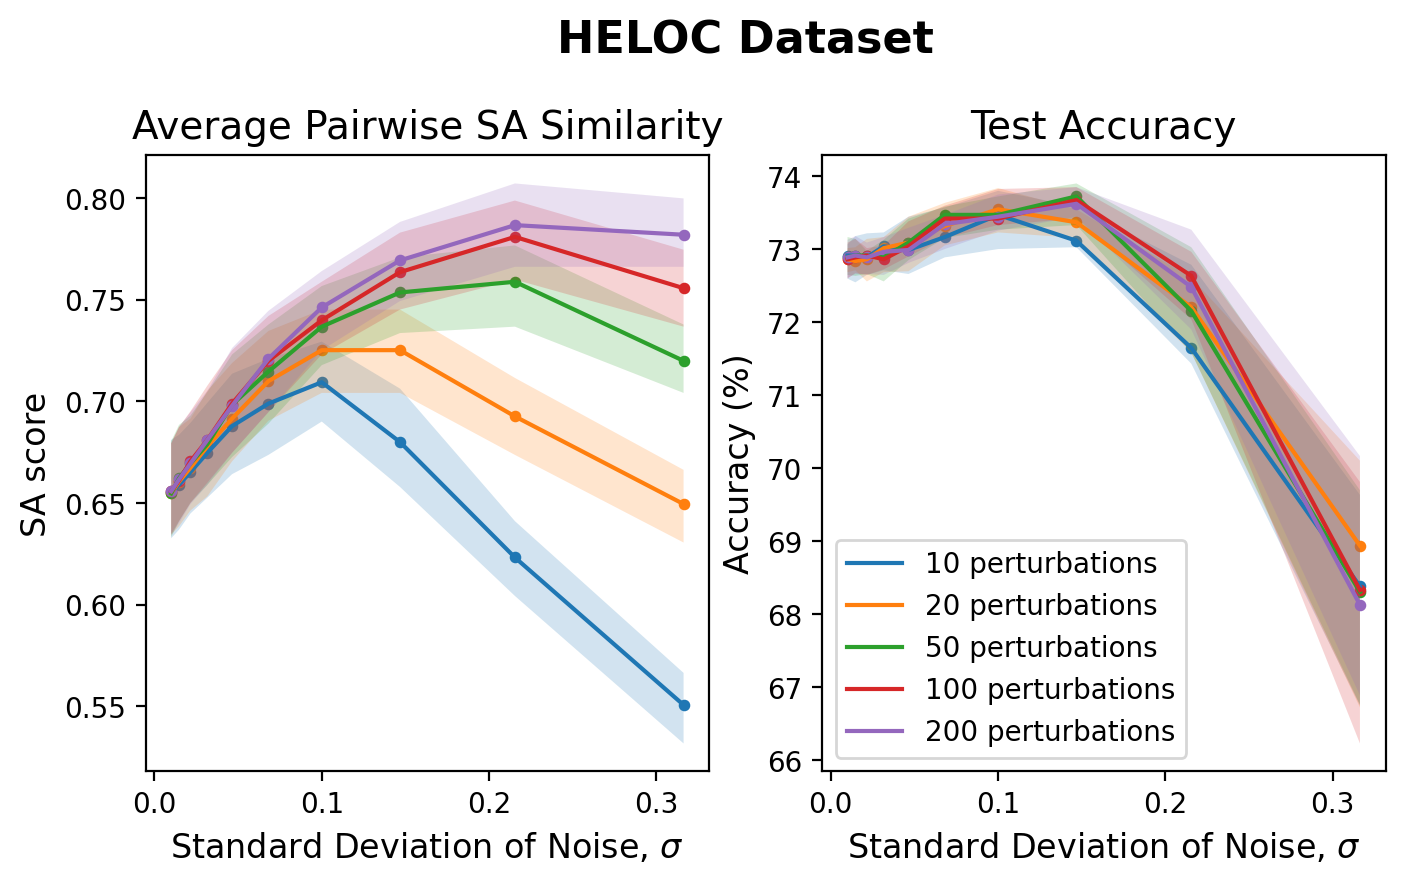
\includegraphics[width=0.325\textwidth]{figures/perturb_heloc_samples.png}
    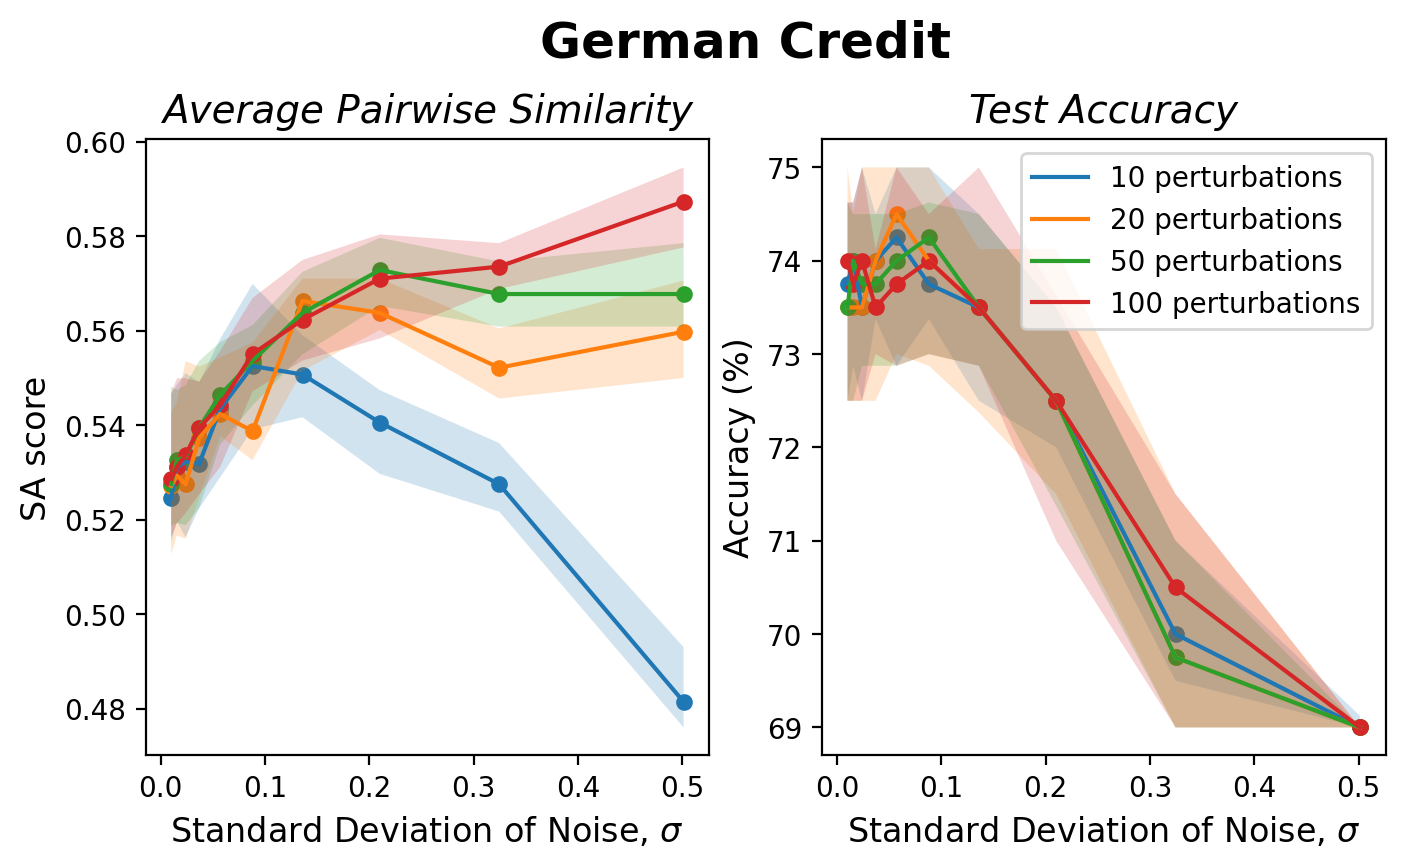
\includegraphics[width=0.325\textwidth]{figures/perturb_german_samples.png}
    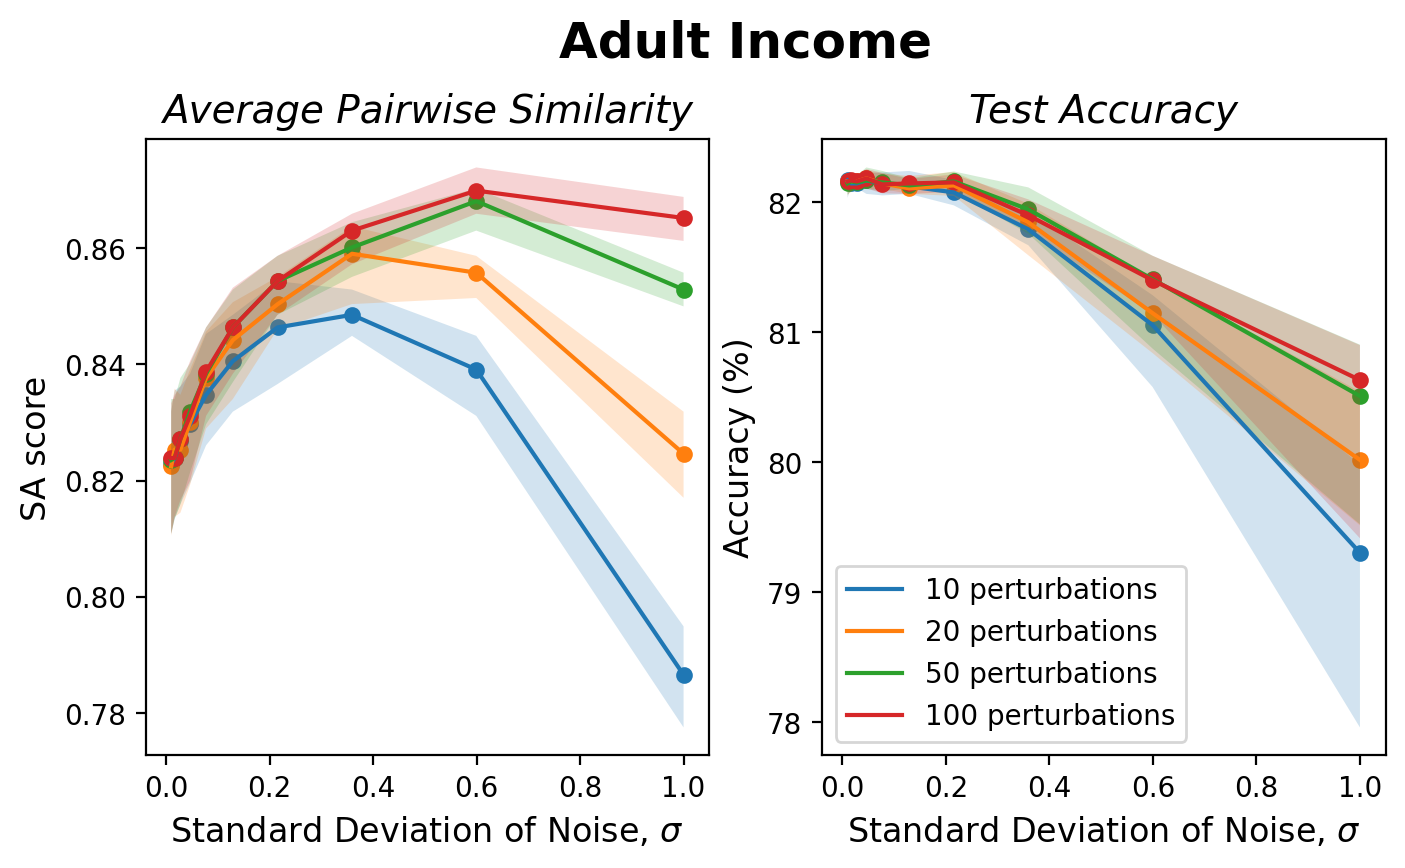
\includegraphics[width=0.325\textwidth]{figures/perturb_adult_samples.png}
    \caption{\small Effect of $\sigma$ on top-k SA scores (for input gradients and $k=5$), and test set accuracy, for an increasing number of perturbations. \textbf{Left to Right:} HELOC, German Credit, and Adult Income datasets, with noise added to first layer biases,  weights, and weights, respectively. Observe how explanation similarity may continually increase, even as test accuracy drops (one is not a strong indicator of the other). Error bars represent the central decile of SA scores over 1000 individuals, and the interquartile ranges of accuracies over perturbed models.}
    \label{fig:perturb_ablation}
\end{figure}

\begin{figure}[t]
    \centering
    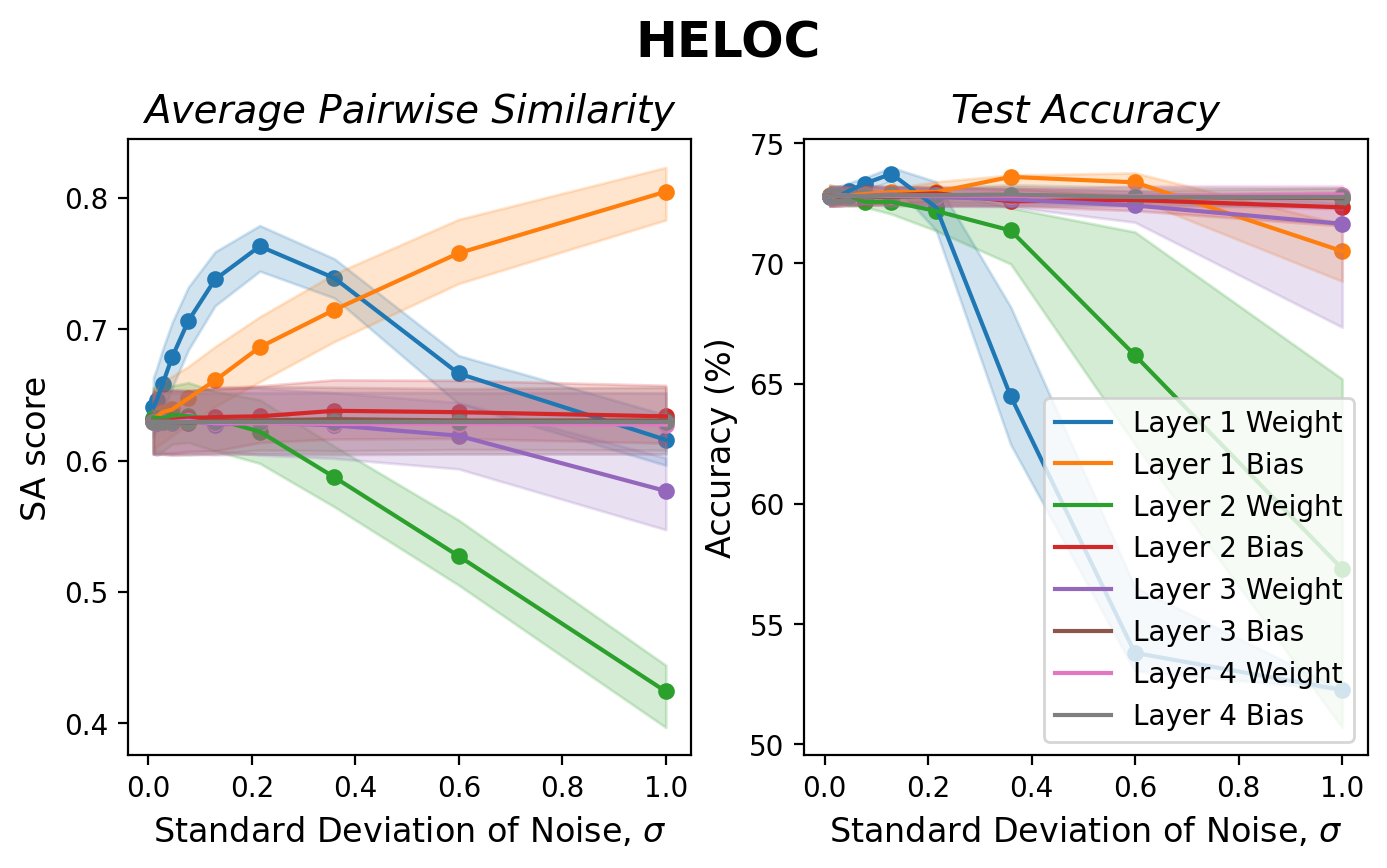
\includegraphics[width=0.325\textwidth]{figures/perturb_heloc_layers.png}
    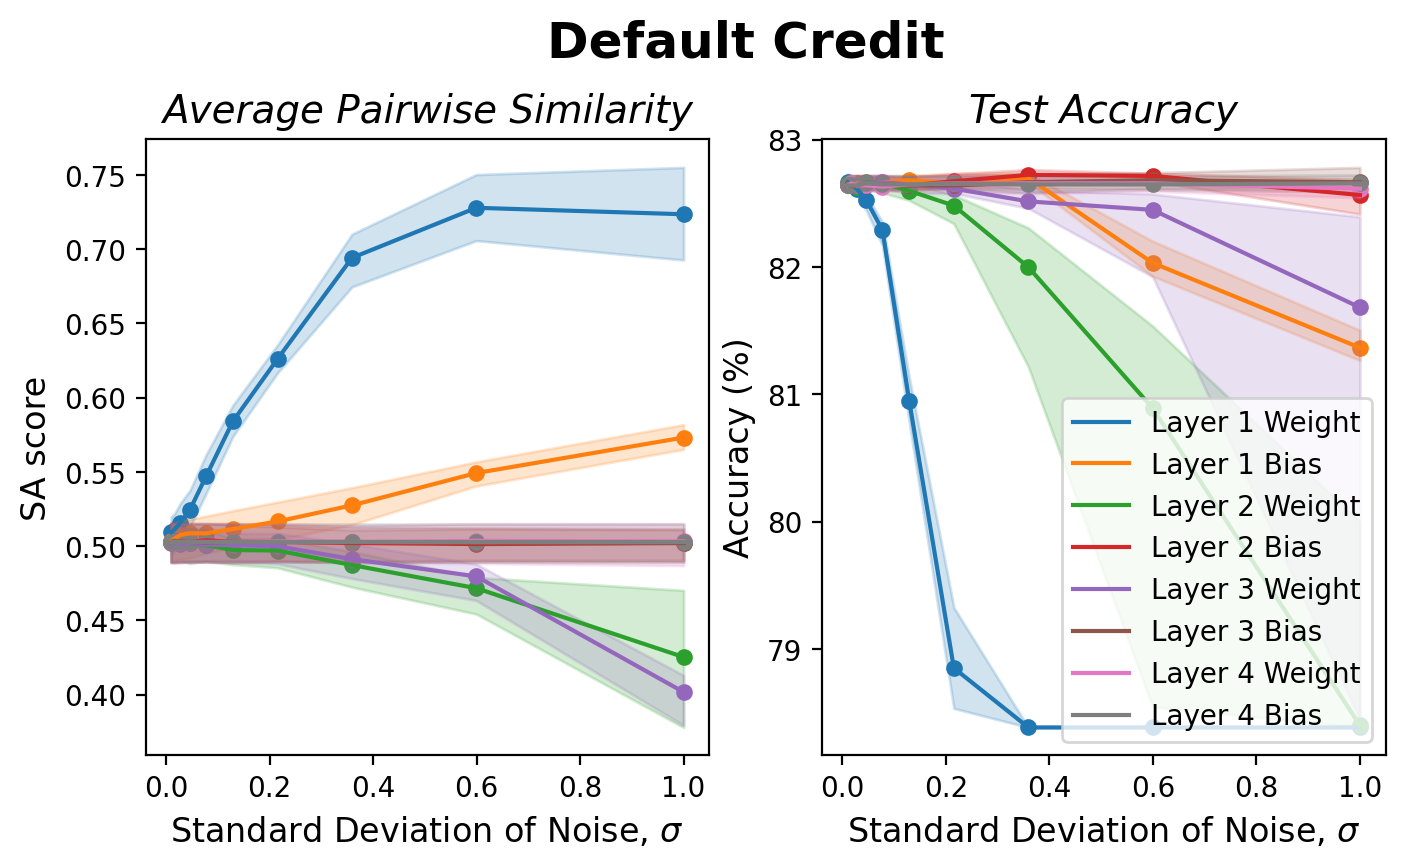
\includegraphics[width=0.325\textwidth]{figures/perturb_default_layers.png}
    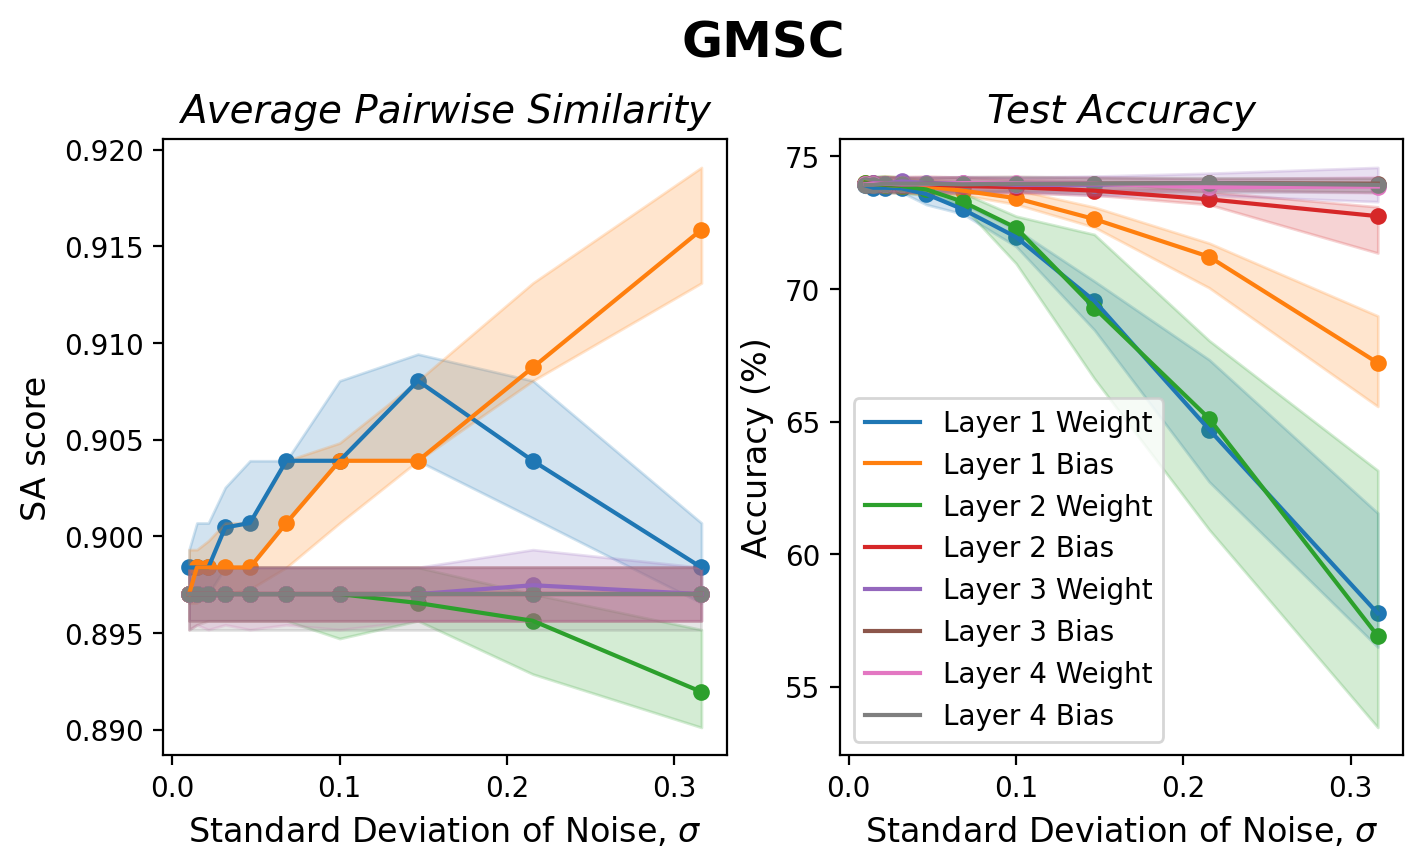
\includegraphics[width=0.325\textwidth]{figures/perturb_gmsc_layers.png}
    \caption{\small Effect of $\sigma$ on top-k SA scores (for input gradients and $k=5$) and test accuracy, over different layers perturbed 100 times. \textbf{Left to Right:} HELOC, Default Credit, and GMSC. Error bars represent the central decile of SA scores over 1000 individuals, and the interquartile range of accuracies over perturbed models.}
    \label{fig:perturb}
\end{figure}

% \subsection{Vanilla ensembles}

% Short (optional) subsection demonstrating that vanilla ensemble techniques (average, majority vote) can achieve near perfect explanation similarity, though require a large number of constituent models.

\subsection{Impact of weight perturbation}
\label{subsec:experiments_weight}

We begin by performing ablations over the value of $\sigma$ used in our weight perturbation method, conducted on 24 models sampled without replacement from the underspecification set of 1000 pre-trained models. Each model is perturbed a number of times, yielding 24 \textit{perturbed models} (a form of ensemble generated from just one pre-trained model, described in \S\ref{subsec:ensembles_weight}). We measure the SA similarity of the top-5 gradient features between all $\binom{24}{2}$ = 276 unique pairs of perturbed models, averaging over all pairs, i.e. error bars correspond to the first 1000 individuals in the test set. Test accuracy is computed over \textit{all} test inputs, with errors bars corresponding to the 24 perturbed models.

These experiments aim to ascertain the impact of local weight perturbations on explanation similarity and test accuracy, thereby informing the optimal setup for our weight perturbation method. Figure~\ref{fig:perturb_ablation} indicates that perturbing the weights or biases of the first layer with Gaussian noise $\epsilon \sim\mathcal{N}(0,\sigma^2)$ can lead to significant increases in explanation similarity (measure between perturbed models). For instance, over values of $\sigma$ where test accuracy remains approximately constant, SA scores on HELOC increase from around 0.62 to 0.74, by perturbing just 20 times the biases of the first layer (in general, convergence required fewer perturbations when perturbing biases compared to weights). Furthermore, these gains correspond to perturbing just a single model. The cumulative effect of constructing ensembles from multiple perturbed models, discussed in \S\ref{subsec:experiments_ensemble}, leads to additional gains. 

We also investigate the effects of perturbing individually each layer of the network (Figure~\ref{fig:perturb}), finding that improvements in explanation similarity \textit{depend critically on the layer being perturbed}\footnote{For clarity, our naming convention is such that \textit{Layer 1} refers to the weights or biases between the input and the first hidden layer, \textit{Layer 2} refers to the weights/biases between the first and second hidden layers, etc.}. Across all datasets, we observe that the weights or biases of the first layer tend to be most sensitive to perturbations, providing potential for improved explanation similarity. For instance, at no point in Figure~\ref{fig:perturb} do SA scores significantly increase when perturbing weights/biases beyond the first layer. Further investigations, including full ablations across all datasets, are located in Appendix~\ref{app:weights}.

% We observe in our experiments that constant loss between two pre-trained models does not necessarily always \textit{guarantee} explanation similarity upon ensembling. Mention of diverse modes discovered between endpoints.


\begin{figure}
    \centering
    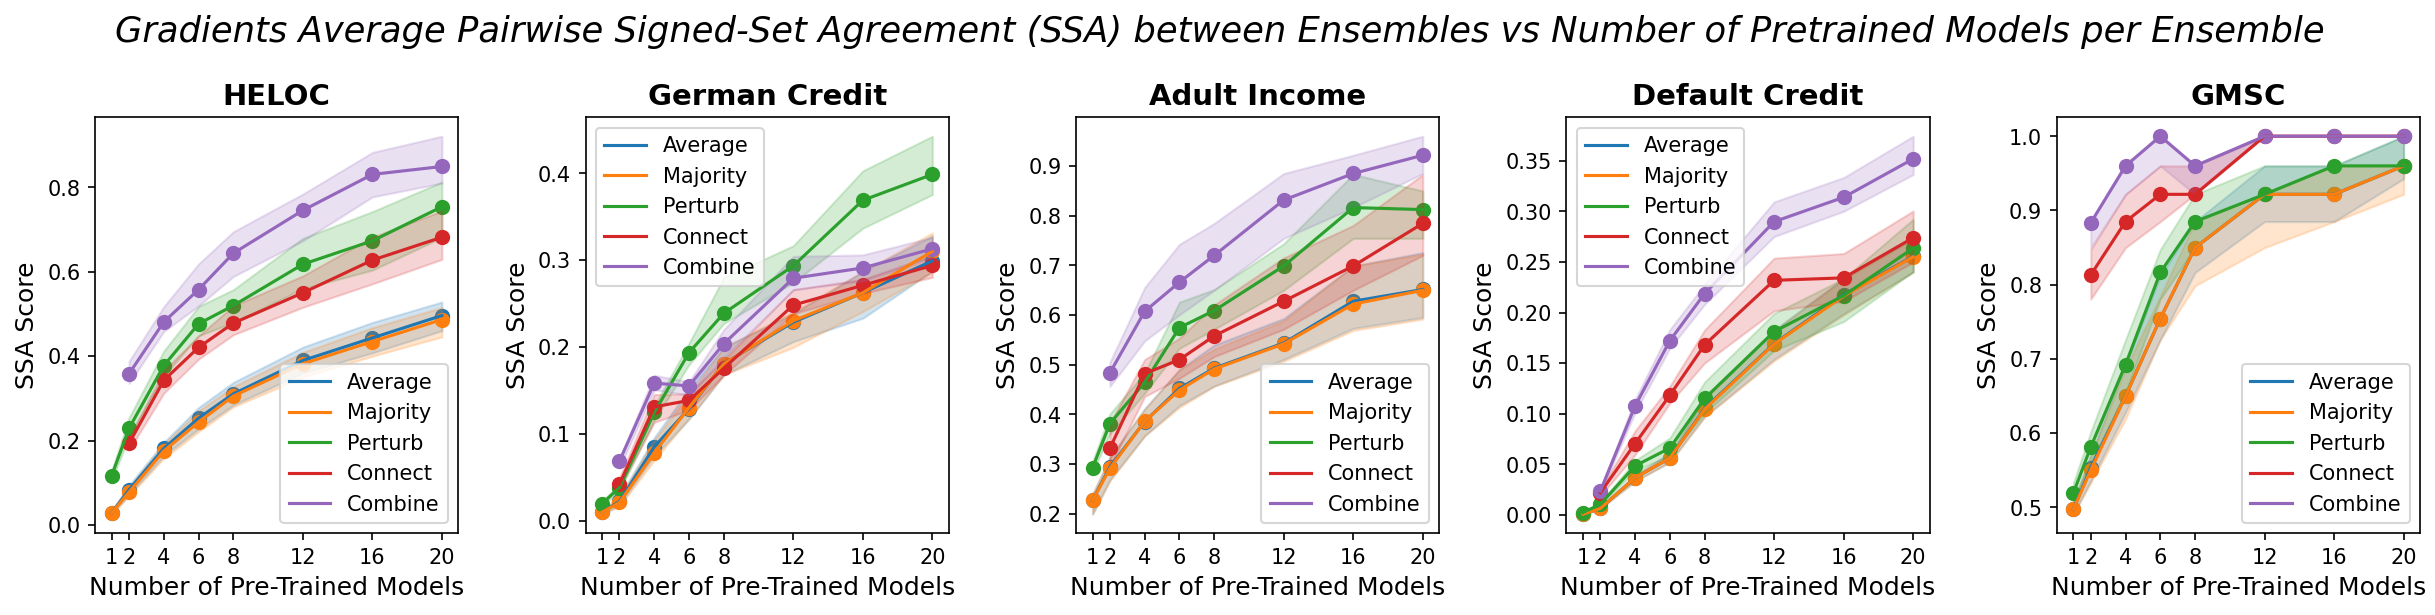
\includegraphics[width=0.99\textwidth]{figures/ssa_top5_gradients.png}
    \caption{\small Effectiveness of ensemble strategies in stabilizing explanations across all datasets (top-5 SSA scores for input gradients). Observe the increases in similarity between ensembles when combining global (mode connectivity) and local (perturbation) explorations. \textit{Average} and \textit{Majority} denote vanilla ensembles, while \textit{Perturb}, \textit{Connect}, and \textit{Combine} denote weight perturbation, mode connectivity, and their combination.}% respectively.}
    \label{fig:ensembles}
\end{figure}

\subsection{Comparison of ensemble techniques}
\label{subsec:experiments_ensemble}

In our experiments, we construct ensembles by randomly sampling 50 non-overlapping sets of models from the underspecification set of 1000 pre-trained models. The size of each set differs per experiment, with a maximum size of 20 pre-trained models (covering all 1000 models). For a given $k$ value and explanation technique, we then compute similarity scores between all $\binom{50}{2}$ = 1225 unique pairs of ensembles, averaging over all pairs. Thus, scores represent the range of probability values that individuals have of satisfying certain similarity criteria. For example, SSA scores estimate the likelihood that individuals maintain identical top-$k$ features (i.e. with the same directions, but ignoring ordering), when switching between approximately equivalent models.

We also trial the combination of both weight perturbation (\textit{perturb}) and mode connectivity (\textit{connect}), as a novel ensembling technique (denoted \textit{combine}), which involves uniformally sampling models along each mode connecting path, and perturbing each of them. Full results across all datasets, explanation methods, and similarity metrics are provided in Appendix~\ref{app:experiments}.

% Explain average, majority, perturb, connect, combine. (in figure too) novel

\paragraph{Vanilla ensembles can eliminate explanatory multiplicity, when sufficiently large} Whether the distribution of model explanations across the underspecification set has low or high variance, the explanations between vanilla ensembles of sufficient size sampled from the set will eventually converge. We observe this convergence in Figure~\ref{fig:ensembles}. While vanilla ensembles of just 20 pre-trained models cannot achieve perfect similarity in all cases, as the ensembles grow in size we see a steady increase in average pairwise SSA score (the strictest criterion). For the GMSC dataset, and vanilla ensembles (blue and orange), the median probability of an individual retaining the exact same top-$k$ features when switching between models increases from 50\% to 95\%.

\paragraph{Strategic ensembling reduces pre-training requirements} We demonstrate in Figure~\ref{fig:ensembles} that our ensemble strategies consistently expedite the alignment of model explanations i.e., require fewer pre-trained models to achieve a given similarity score. The relative performance gains that we achieve through either local (green) or global (red) exploration often hinge upon the unique
characteristics of the given dataset, explanation technique, or model class used. We observe that our approach of combining both forms of exploration achieves superior performance in most cases. Notably, to increase SSA scores to around 40\% in HELOC, from 0\% for single models, vanilla ensembles required 12 pre-trained models (blue and orange). Conversely, the combined exploration of mode connectivity and weight perturbation required just 2 pre-trained models (purple). Similarly, the number of pre-trained models required to surpass SSA scores of 60\% on Adult Income, can be reduced fivefold from 20 to just 4. Table~\ref{tab:all_res} showcases further examples in which our methods comprehensively improve explanation similarity across SA, SSA and CDC metrics, for ensembles constructed with four pre-trained models. Note that the CDC metric typically returned 1 for top-5 explanations, and is the least strict of the three metrics. Thus, we instead consider top-$d$ CDC, computing CDC over all $d$ features in the dataset, to stress-test the performance of our ensembling approaches. In this case, we retain significant improvements over vanilla ensembles.

% In Table~\ref{tab:all_res}, ... \dan{(note for now: d is all features- intuitively, this means that CDC is 1 iff all features have the same sign in both models. if we use top-5, scores are normally all just 1.0... perhaps an intermediary value can be justified}.

\paragraph{Ensembling increases test accuracy} A well known property of ensembles is their ability to reduce generalization error \citep{dietterich2000, allenzhu2023}, and we observe the same results in our experiments. Our value of $\sigma$ was chosen to maximize similarity improvements, but with the constraint that the test accuracy does not drop by more than 1\%. In most cases, our ensembling methods achieved similar test accuracies to vanilla ensembles, with test accuracy exceeding standard ensembles by up to 1\% in some cases.

\begin{table*}[t]
\caption{\small Results of explanation alignment for Smoothgrad and DeepSHAP, across all datasets and similarity metrics. Ensembles are constructed from just four pre-trained models. Explanation agreement between \textit{single} models sampled from the underspecification set are shown for reference. We report mean values alongside standard deviation. Best values are shown in bold.}
\label{tab:all_res}
\centering
\fontsize{8}{7}\selectfont
\begin{tabular}{ccccccccc}\toprule
\multirow{2}{*}{\textit{Dataset}} & \multirow{2}{*}{\parbox{0.08\textwidth}{\centering\textit{Ensemble Method}}} & \multicolumn{3}{c}{\textit{-------------------- Smoothgrad --------------------}} & \multicolumn{3}{c}{\textit{--------------------- DeepSHAP -----------------------}} \\
& & \textit{Top-5 SA} & \textit{Top-5 SSA} & \textit{Top-d CDC} & \textit{Top-5 SA} & \textit{Top-5 SSA} & \textit{Top-d CDC} \\\midrule
\multirow{5}{*}{\parbox{0.09\textwidth}{\centering\textbf{HELOC}\\ \scriptsize (23 features)}}
    & \textit{Single} & \textit{0.65 $\pm$ 0.09} & \textit{0.06 $\pm$ 0.06} & \textit{0.01 $\pm$ 0.01} & \textit{0.75 $\pm$ 0.09} & \textit{0.18 $\pm$ 0.17} & \textit{0.02 $\pm$ 0.02} \\
    & Vanilla & 0.81 $\pm$ 0.08 & 0.25 $\pm$ 0.19 & 0.09 $\pm$ 0.09 & 0.84 $\pm$ 0.09 & 0.39 $\pm$ 0.27 & 0.09 $\pm$ 0.09 \\
    & Perturb & 0.87 $\pm$ 0.06 & 0.43 $\pm$ 0.23 & 0.19 $\pm$ 0.14 & 0.86 $\pm$ 0.07 & 0.44 $\pm$ 0.23 & 0.12 $\pm$ 0.08 \\
    & Connect & 0.86 $\pm$ 0.07 & 0.39 $\pm$ 0.22 & 0.15 $\pm$ 0.13 & 0.88 $\pm$ 0.08 & 0.51 $\pm$ 0.28 & 0.11 $\pm$ 0.10 \\
    & Combine & \textbf{0.90 $\pm$ 0.06} & \textbf{0.55 $\pm$ 0.25} & \textbf{0.26 $\pm$ 0.17} & \textbf{0.90 $\pm$ 0.07} & \textbf{0.55 $\pm$ 0.28} & \textbf{0.14 $\pm$ 0.10} \\ \midrule
\multirow{5}{*}{\parbox{0.09\textwidth}{\centering\textbf{German\\Credit}\\ \scriptsize (70 features)}}
    & \textit{Single} & \textit{0.50 $\pm$ 0.08} & \textit{0.01 $\pm$ 0.01} & \textit{0.00 $\pm$ 0.00} & \textit{0.68 $\pm$ 0.11} & \textit{0.11 $\pm$ 0.15} & \textit{0.00 $\pm$ 0.00} \\
    & Vanilla & 0.69 $\pm$ 0.08 & 0.09 $\pm$ 0.07 & 0.00 $\pm$ 0.00 & 0.80 $\pm$ 0.09 & 0.27 $\pm$ 0.24 & 0.00 $\pm$ 0.00 \\
    & Perturb & 0.73 $\pm$ 0.07 & 0.12 $\pm$ 0.08 & 0.00 $\pm$ 0.00 & \textbf{0.83 $\pm$ 0.08} & \textbf{0.32 $\pm$ 0.22} & 0.00 $\pm$ 0.00 \\
    & Connect & 0.71 $\pm$ 0.12 & 0.12 $\pm$ 0.10 & 0.00 $\pm$ 0.00 & 0.77 $\pm$ 0.10 & 0.22 $\pm$ 0.21 & 0.00 $\pm$ 0.00 \\
    & Combine & \textbf{0.76 $\pm$ 0.08} & \textbf{0.17 $\pm$ 0.12} & 0.00 $\pm$ 0.00 & 0.81 $\pm$ 0.08 & 0.27 $\pm$ 0.21 & 0.00 $\pm$ 0.00 \\ \midrule
\multirow{5}{*}{\parbox{0.09\textwidth}{\centering\textbf{Adult\\Income}\\ \scriptsize (6 features)}}
    & \textit{Single} & \textit{0.83 $\pm$ 0.07} & \textit{0.29 $\pm$ 0.18} & \textit{0.32 $\pm$ 0.15} & \textit{0.92 $\pm$ 0.07} & \textit{0.63 $\pm$ 0.31} & \textit{0.51 $\pm$ 0.17} \\
    & Vanilla & 0.89 $\pm$ 0.06 & 0.48 $\pm$ 0.24 & 0.50 $\pm$ 0.19 & 0.95 $\pm$ 0.06 & 0.75 $\pm$ 0.26 & 0.66 $\pm$ 0.20 \\
    & Perturb & 0.90 $\pm$ 0.05 & 0.54 $\pm$ 0.24 & 0.54 $\pm$ 0.19 & 0.95 $\pm$ 0.05 & 0.77 $\pm$ 0.23 & 0.77 $\pm$ 0.19 \\
    & Connect & 0.90 $\pm$ 0.07 & 0.53 $\pm$ 0.27 & 0.53 $\pm$ 0.22 & 0.96 $\pm$ 0.05 & 0.79 $\pm$ 0.24 & 0.74 $\pm$ 0.20 \\
    & Combine & \textbf{0.92 $\pm$ 0.06} & \textbf{0.61 $\pm$ 0.26} & \textbf{0.58 $\pm$ 0.21} & \textbf{0.96 $\pm$ 0.04} & \textbf{0.81 $\pm$ 0.21} & \textbf{0.78 $\pm$ 0.20} \\\midrule
\multirow{5}{*}{\parbox{0.09\textwidth}{\centering\textbf{Default\\Credit}\\ \scriptsize (90 features)}}
    & \textit{Single} & \textit{0.49 $\pm$ 0.06} & \textit{0.00 $\pm$ 0.00} & \textit{0.00 $\pm$ 0.00} & \textit{0.82 $\pm$ 0.07} & \textit{0.29 $\pm$ 0.18} & \textit{0.00 $\pm$ 0.00} \\
    & Vanilla & 0.67 $\pm$ 0.07 & 0.04 $\pm$ 0.04 & 0.01 $\pm$ 0.02 & 0.89 $\pm$ 0.07 & 0.54 $\pm$ 0.27 & 0.02 $\pm$ 0.04 \\
    & Perturb & 0.72 $\pm$ 0.06 & 0.07 $\pm$ 0.07 & 0.02 $\pm$ 0.03 & 0.90 $\pm$ 0.07 & 0.54 $\pm$ 0.27 & 0.03 $\pm$ 0.04 \\
    & Connect & 0.70 $\pm$ 0.07 & 0.07 $\pm$ 0.05 & 0.02 $\pm$ 0.03 & 0.91 $\pm$ 0.06 & 0.58 $\pm$ 0.25 & 0.03 $\pm$ 0.03 \\
    & Combine & \textbf{0.75 $\pm$ 0.05} & \textbf{0.11 $\pm$ 0.05} & \textbf{0.03 $\pm$ 0.06} & \textbf{0.91 $\pm$ 0.06} & \textbf{0.58 $\pm$ 0.25} & \textbf{0.03 $\pm$ 0.02} \\ \midrule
\multirow{5}{*}{\parbox{0.09\textwidth}{\centering\textbf{GMSC}\\ \scriptsize (10 features)}}
    & \textit{Single} & \textit{0.91 $\pm$ 0.03} & \textit{0.57 $\pm$ 0.15} & \textit{0.46 $\pm$ 0.23} & \textit{0.85 $\pm$ 0.07} & \textit{0.39 $\pm$ 0.21} & \textit{0.39 $\pm$ 0.19} \\
    & Vanilla & 0.95 $\pm$ 0.04 & 0.75 $\pm$ 0.19 & 0.67 $\pm$ 0.25 & 0.90 $\pm$ 0.07 & 0.60 $\pm$ 0.25 & 0.58 $\pm$ 0.22 \\
    & Perturb & 0.95 $\pm$ 0.04 & 0.76 $\pm$ 0.19 & 0.69 $\pm$ 0.24 & 0.90 $\pm$ 0.07 & 0.60 $\pm$ 0.25 & 0.59 $\pm$ 0.21 \\
    & Connect & 0.96 $\pm$ 0.04 & 0.82 $\pm$ 0.18 & 0.71 $\pm$ 0.25 & 0.90 $\pm$ 0.06 & 0.58 $\pm$ 0.25 & 0.62 $\pm$ 0.20 \\
    & Combine & \textbf{0.97 $\pm$ 0.04} & \textbf{0.83 $\pm$ 0.18} & \textbf{0.72 $\pm$ 0.24} & \textbf{0.91 $\pm$ 0.06} & \textbf{0.62 $\pm$ 0.26} & \textbf{0.66 $\pm$ 0.21} \\ \midrule
\end{tabular}
\end{table*}

% \subsection{Robustness to dataset shift (optional)}

% TBC. Leaning towards omitting this section for space constraints and relevance. The idea is that for small dataset shifts, there is significant disagreement between any one base model, and a number of models sampled from the underspecification set of the shifted data, but that using ensembles can significantly reduce this.



